\begin{figure}[t]
\small{
\centering
\begin{subfigure}[t]{0.48\linewidth}
    \begin{tabular}{cc}
    %
    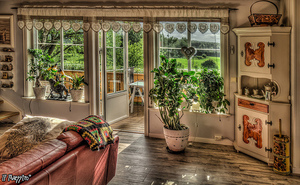
\includegraphics[width=.43\linewidth]{../../figures/flickrDatasetExamples/used/resized/hdr.jpg} &
    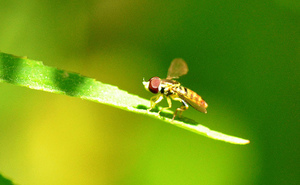
\includegraphics[width=.43\linewidth]{../../figures/flickrDatasetExamples/used/resized/macro.jpg} \\
    HDR & Macro \\
    %
    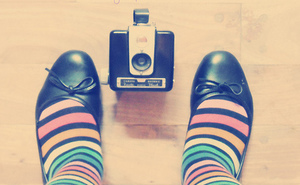
\includegraphics[width=.43\linewidth]{../../figures/flickrDatasetExamples/used/resized/vintage.jpg} &
    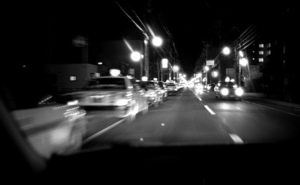
\includegraphics[width=.43\linewidth]{../../figures/flickrDatasetExamples/used/resized/noir.jpg} \\
    Vintage & Noir \\
    %
    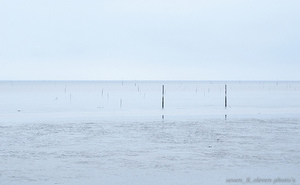
\includegraphics[width=.43\linewidth]{../../figures/flickrDatasetExamples/used/resized/minimal.jpg} &
    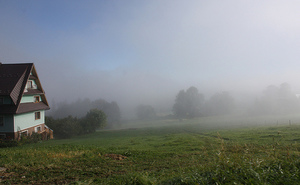
\includegraphics[width=.43\linewidth]{../../figures/flickrDatasetExamples/used/resized/hazy.jpg} \\
    Minimal & Hazy \\
    %
    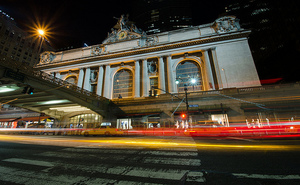
\includegraphics[width=.43\linewidth]{../../figures/flickrDatasetExamples/used/resized/long_exposure.jpg} &
    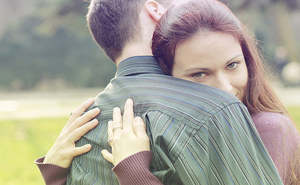
\includegraphics[width=.43\linewidth]{../../figures/flickrDatasetExamples/used/resized/romantic.jpg} \\
    Long Exposure & Romantic \\
    \end{tabular}
    \caption{
        Flickr Style: 80K images covering 20 styles.
    }\label{fig:flickr_style_examples}
\end{subfigure}%
\hspace{2em}%
\begin{subfigure}[t]{0.48\linewidth}
    \begin{tabular}{cc}
    %
    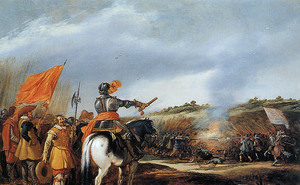
\includegraphics[width=.43\linewidth]{../../figures/wikipaintingsDatasetExamples/used/resized/baroque-0.jpg} &
    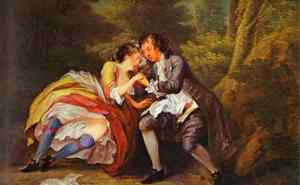
\includegraphics[width=.43\linewidth]{../../figures/wikipaintingsDatasetExamples/used/resized/roccoco-0.jpg} \\
    Baroque & Roccoco \\
    %
    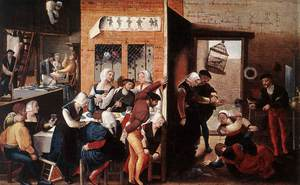
\includegraphics[width=.43\linewidth]{../../figures/wikipaintingsDatasetExamples/used/resized/northern_renaissance-0.jpg} &
    % NOTE: ukiyoe-0 is messing up for unknown reason
    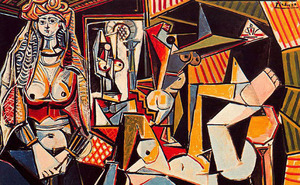
\includegraphics[width=.43\linewidth]{../../figures/wikipaintingsDatasetExamples/used/resized/cubism-0.jpg} \\
    Northern Renaissance & Cubism \\
    %
    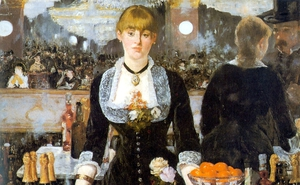
\includegraphics[width=.43\linewidth]{../../figures/wikipaintingsDatasetExamples/used/resized/impressionism-0.jpg} &
    % NOTE: post-impressionism was messing up until I output it as png
    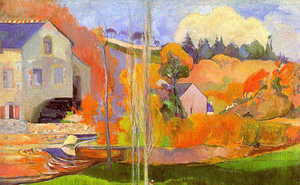
\includegraphics[width=.43\linewidth]{../../figures/wikipaintingsDatasetExamples/used/resized/post_impressionism-0.jpg} \\
    Impressionism & Post-Impressionism \\
    %
    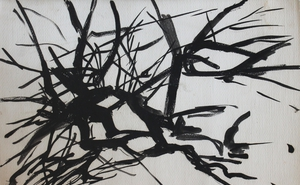
\includegraphics[width=.43\linewidth]{../../figures/wikipaintingsDatasetExamples/used/resized/abs_expressionism-0.jpg} &
    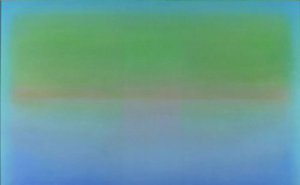
\includegraphics[width=.43\linewidth]{../../figures/wikipaintingsDatasetExamples/used/resized/color_field-0.jpg} \\
    Abs. Expressionism & Color Field Painting \\
    \end{tabular}
    \caption{
        Wikipaintings: 85K images for 25 art genres.
    }\label{fig:wikipaintings_style_examples}
\end{subfigure}
}
\caption{
    Typical images in different style categories of our datasets.
}\label{fig:style_examples}
\end{figure}
